\documentclass[tikz,border=2pt]{standalone}
\usepackage{amsmath,amssymb}
\usepackage{xcolor}
\usetikzlibrary{positioning}
\begin{document}
% Extracted from namuenofull.inc; source column: \footnotesize \cite{NU}$_{\rm p{ 166 }}$ IV$^*$-IV$^*$-$\alpha$
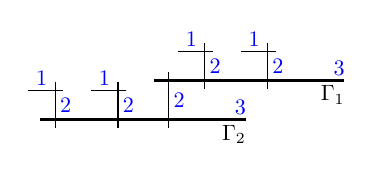
\begin{tikzpicture}[xscale=0.57,yscale=0.62]
\draw[thick,shorten >=2] (4/15,0)--(149/30,0) node[inner sep=2pt,blue,above left,scale=0.8] {3} node[inner sep=2pt,below left,scale=0.8] {$\Gamma_2$};
\draw[shorten <=-3pt, shorten >=-3pt] (3/5,0)--node[inner sep=2pt,scale=0.8,blue,right] {2} (3/5,3/5);
\draw[shorten <=-3pt] (3/5,3/5)--node[inner sep=2pt,scale=0.8,blue,above] {1} (0,3/5);
\draw[shorten <=-3pt, shorten >=-3pt] (2,0)--node[inner sep=2pt,scale=0.8,blue,right] {2} (2,3/5);
\draw[shorten <=-3pt] (2,3/5)--node[inner sep=2pt,scale=0.8,blue,above] {1} (7/5,3/5);
\draw[shorten <=-3pt, shorten >=-3pt] (47/15,0)--node[inner sep=2pt,scale=0.8,blue,right] {2} (47/15,4/5);
\draw[thick,shorten >=2] (14/5,4/5)--(43/6,4/5) node[inner sep=2pt,blue,above left,scale=0.8] {3} node[inner sep=2pt,below left,scale=0.8] {$\Gamma_1$};
\draw[shorten <=-3pt, shorten >=-3pt] (59/15,4/5)--node[inner sep=2pt,scale=0.8,blue,right] {2} (59/15,7/5);
\draw[shorten <=-3pt] (59/15,7/5)--node[inner sep=2pt,scale=0.8,blue,above] {1} (10/3,7/5);
\draw[shorten <=-3pt, shorten >=-3pt] (16/3,4/5)--node[inner sep=2pt,scale=0.8,blue,right] {2} (16/3,7/5);
\draw[shorten <=-3pt] (16/3,7/5)--node[inner sep=2pt,scale=0.8,blue,above] {1} (71/15,7/5);
\end{tikzpicture}
\end{document}
